\documentclass[11pt]{article} % type of the document
\usepackage[english]{babel} % language of all the auto generated text
\usepackage{lmodern} % use a high quality font
\usepackage{listings} % include code snippets
\usepackage{color} % use colors
\usepackage{textcomp} % additional symbols
\usepackage[hyphens]{url} % adds the \url command
\usepackage[hidelinks]{hyperref}
\usepackage{graphicx} % used for graphics stuff
\usepackage{subcaption} % allows adding subfigures
\usepackage{fancyhdr} % header and footer
\usepackage{todonotes} % \todo command
\usepackage{everypage} % run stuff on every page
\usepackage{pdfpages} % include pdf files as figures
\usepackage[noindentafter]{titlesec}
\usepackage{xspace} % add spaces after macros if necessary
\usepackage{amstext} % includes the \text command
\usepackage{booktabs} % table styling
\usepackage{lipsum} % lorem ipsum
\usepackage{enumitem}
\usepackage{float} % absolute positioning of floats
\usepackage{amsfonts} % additional fonts (used for \textbb
\usepackage{booktabs} % table styling
\usepackage{longtable} % repeat table header on each page
\usepackage{xspace} % used to correct spacing after abbreviations
\usepackage{amssymb,array}
\usepackage{enumitem}
\usepackage{geometry} % define the geometry of the page
\geometry{a4paper,left=25mm,right=25mm, top=28mm, bottom=28mm} 

\setcounter{tocdepth}{5} % define the depth of the table of contents
\setcounter{secnumdepth}{5} % define the depth of the section structure

% paragraphs look like subsubsubsections
\titleformat{\paragraph}[hang]{\bf}{\thetitle\quad}{0pt}{}
\titlespacing{\paragraph}{0pt}{1em}{0.5em} 

% subparagraphs look like paragraphs used to look
\titleformat{\subparagraph}[runin]{\bf}{}{0.5em}{}
\titlespacing{\subparagraph}{0pt}{1em}{1em}

\newcommand{\Ra}{\ensuremath{\Rightarrow}\xspace}
\newcommand{\ra}{\ensuremath{\rightarrow}\xspace}

\definecolor{dark-gray}{gray}{0.3}

\newcommand{\floatright}[1]{\hfill \textcolor{dark-gray}{#1}}

% adds a foot rule to every page
\AddEverypageHook
{
    \renewcommand{\footrulewidth}{0.4pt}
}

% define escape characters for latex commands in listings
\lstset{%
  escapeinside={(*}{*)},%
}

% define symbols for optional and non-optional properties
\newcommand{\nonoptional}{\ensuremath{{}^{\textbf{\circ}}}}
\newcommand{\nonoptionalif}{\ensuremath{{}^{\textbf{*}}}}

% define minipage in tabular
\newcommand{\cellwrap}[1]{\begin{minipage}[t]{1.0\columnwidth}#1\end{minipage}}

% define abbreviations properly
\newcommand*{\eg}{e.g.\@\xspace}
\newcommand*{\ie}{i.e.\@\xspace}

\newcommand{\pipe}{\ensuremath{|}\xspace}

% define colored text method
\newcommand{\coloredtext}[1]{\color[HTML]{#1}{\##1}}

\renewcommand{\thesubfigure}{\Alph{subfigure}}

%%%%%%%%%% DEFINE VARIABLES HERE %%%%%%%%%%%%%%%
\newcommand{\instanceStuff}{\texttt{instance-stuff}}


%%%%%%%%%% TIKZ DEFINITIONS %%%%%%%%%%%%


% style the header and footer
\pagestyle{fancy}
\renewcommand{\sectionmark}[1]{\markright{#1}}
\fancyfoot[R]{\thepage}
\fancyfoot[C]{}
\fancyhead[L]{Germinate 3}
\fancyhead[R]{\nouppercase{\rightmark}}

\hypersetup{
	pdfauthor={Sebastian Raubach},
	pdftitle={Germinate 3 User Guide},
	pdfinfo={Copyright={Copyright 2013-\the\year The James Hutton Institute. All rights reserved.}}
}

\makeatletter
\lst@CCPutMacro\lst@ProcessOther {"2D}{\lst@ttfamily{-{}}{-{}}}
\@empty\z@\@empty
\makeatother

% the document starts here
\begin{document}

% remove page numbers for title and TOC
\pagenumbering{gobble}
% title page is compiled by itself
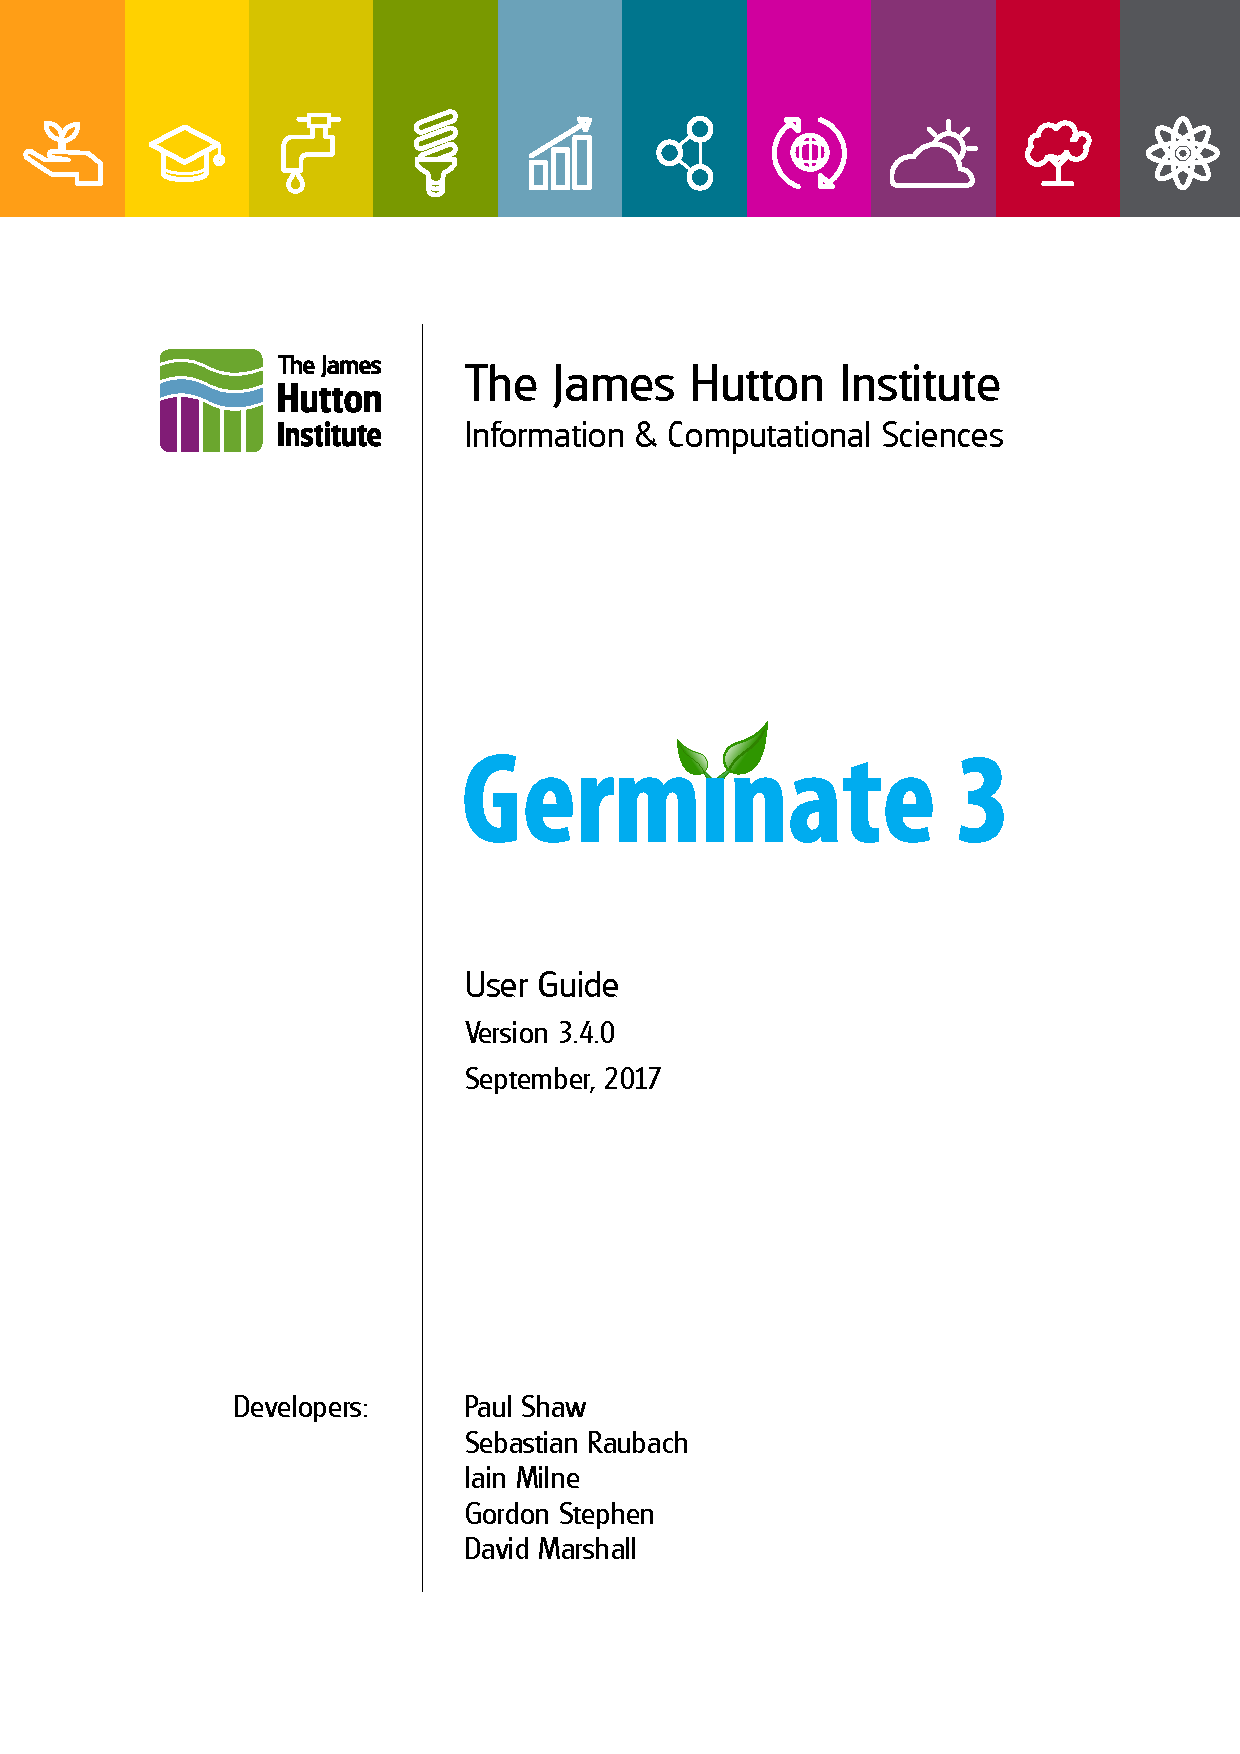
\includepdf{title.pdf}

% add the table of contents
\tableofcontents

% Include the styling of the code snippets
%\include{theme-dark}
% code styling for java
\lstdefinestyle{Java}{
	backgroundcolor=\color[RGB]{240,240,240},
	tabsize=4,
	rulecolor=\color[RGB]{200,200,200},
    frame=tblr,
    framerule=0.1pt,
    framexleftmargin=0pt,
	language=java,
    basicstyle=\scriptsize\color[rgb]{0,0,0},
    upquote=true,
    aboveskip={0.5\baselineskip},
    columns=fullflexible,
    showstringspaces=false,
    extendedchars=true,
    breaklines=true,
    prebreak=,
    showtabs=false,
    showspaces=false,
    showstringspaces=false,
    identifierstyle=\ttfamily,
    keywordstyle=\color[RGB]{32,96,160},
    commentstyle=\color[RGB]{70,70,70},
    stringstyle=\color[RGB]{0,153,51},
    morekeywords={@Override,@RemoteServiceRelativePath,@PluralCount},
}

% code styling for javascript
\lstdefinestyle{JavaScript}{
	backgroundcolor=\color[RGB]{240,240,240},
	tabsize=4,
	rulecolor=\color[RGB]{200,200,200},
	frame=tblr,
	framerule=0.1pt,
	framexleftmargin=0pt,
	language=,
	basicstyle=\scriptsize\color[rgb]{0,0,0},
	upquote=true,
	aboveskip={0.5\baselineskip},
	columns=fullflexible,
	showstringspaces=false,
	extendedchars=true,
	breaklines=true,
	prebreak=,
	showtabs=false,
	showspaces=false,
	showstringspaces=false,
	identifierstyle=\ttfamily,
	keywordstyle=\color[RGB]{32,96,160},
	commentstyle=\color[RGB]{70,70,70},
	stringstyle=\color[RGB]{0,153,51},
	keywords={typeof, new, true, false, catch, function, return, null, catch, switch, var, if, in, while, do, else, case, break},
	morestring=[b]",
	morestring=[b]'
}



% code styling for HTML
\lstdefinestyle{HTML}{
	backgroundcolor=\color[RGB]{240,240,240},
	tabsize=4,
	rulecolor=\color[RGB]{200,200,200},
    frame=tblr,
    framerule=0.1pt,
    framexleftmargin=0pt,
	language=java,
    basicstyle=\scriptsize\color[rgb]{0,0,0},
    upquote=true,
    aboveskip={0.5\baselineskip},
    columns=fullflexible,
    showstringspaces=false,
    extendedchars=true,
    breaklines=true,
    prebreak=,
    showtabs=false,
    showspaces=false,
    showstringspaces=false,
    identifierstyle=\ttfamily,
    keywordstyle=\color[RGB]{32,96,160},
    commentstyle=\color[RGB]{70,70,70},
    stringstyle=\color[RGB]{0,153,51},
    morekeywords={},
}

% code styling for the .properties files
\lstdefinestyle{Properties}{
	backgroundcolor=\color[RGB]{240,240,240},
	tabsize=4,
	rulecolor=\color[RGB]{200,200,200},
    frame=tblr,
    framerule=0.1pt,
    framexleftmargin=0pt,
	language=,
    basicstyle=\scriptsize\color[rgb]{0,0,0},
    upquote=true,
    aboveskip={0.5\baselineskip},
    columns=fullflexible,
    showstringspaces=false,
    extendedchars=true,
    breaklines=true,
    prebreak=,
    showtabs=false,
    showspaces=false,
    showstringspaces=false,
    identifierstyle=\ttfamily,
    keywordstyle=\color[RGB]{32,96,160},
    commentstyle=\color[RGB]{70,70,70},
    stringstyle=\color[RGB]{0,153,51},
    morekeywords={Germinate,GerminateGatekeeper,Database,Username,Password,Server,Name,UsePort,Port,UseAuthentication,
    Debug,KeepTemporaryFileForHours,Template,VersionName,VersionLink,VersionImage,VersionNumber,Title,DatabaseName,
    TwitterLink,Copyright,Flapjack,Path,CreateProjectMain,AvailablePages,BaseSearchColumn,menuMyFanyPage,iSeeTrees,
    welcomeMessage,LogoMap,BaseTableExternalLink,BaseTableExternalLinkColumn,CollectingsiteTreemapColumn,CookieLifespanMinutes,
    AlleleFreq,MakeHistogram,CreateImage,BinData,Java,R,Gatekeeper,HighlightColor,Menu,GradientTop,GradientBottom,
    CategoricalColors,GradientColors,EmailAddress,ShowHomeOnLogin,BCrypt,Rounds,Registration,Enabled,Needs,Approval,GoogleAnalytics,TrackingId,
    CookieNotifier,UploadSizeLimitMB,Social,ShowFacebook,ShowTwitter,ShowGooglePlus,URL,Server,Logging,IsUnderMaintenance,
    ExternalDataFolder,HideIdColumns,AccessionDisplayColumn,IsReadOnly,Gallery,Images,Per,Page,UseToggleSwitches,Show,Search,Logo,Contains,Link,Show,Parallax,Banner,CustomMenu}
}

\lstdefinestyle{CSS}{
    backgroundcolor=\color[RGB]{240,240,240},
	tabsize=4,
	rulecolor=\color[RGB]{200,200,200},
    frame=tblr,
    framerule=0.1pt,
    framexleftmargin=0pt,
	language=,
    basicstyle=\scriptsize\color[rgb]{0,0,0},
    upquote=true,
    aboveskip={0.5\baselineskip},
    columns=fullflexible,
    showstringspaces=false,
    extendedchars=true,
    breaklines=true,
    prebreak=,
    showtabs=false,
    showspaces=false,
    showstringspaces=false,
    identifierstyle=\ttfamily,
    keywordstyle=\color[RGB]{32,96,160},
    commentstyle=\color[RGB]{70,70,70},
    stringstyle=\color[RGB]{0,153,51},
    morekeywords={accelerator,azimuth,background,background-attachment,
	    background-color,background-image,background-position,
	    background-position-x,background-position-y,background-repeat,
	    behavior,border,border-bottom,border-bottom-color,
	    border-bottom-style,border-bottom-width,border-collapse,
	    border-color,border-left,border-left-color,border-left-style,
	    border-left-width,border-right,border-right-color,
	    border-right-style,border-right-width,border-spacing,
	    border-style,border-top,border-top-color,border-top-style,
	    border-top-width,border-width,bottom,caption-side,clear,
	    clip,color,content,counter-increment,counter-reset,cue,
	    cue-after,cue-before,cursor,direction,display,elevation,
	    empty-cells,filter,float,font,font-family,font-size,
	    font-size-adjust,font-stretch,font-style,font-variant,
	    font-weight,height,ime-mode,include-source,
	    layer-background-color,layer-background-image,layout-flow,
	    layout-grid,layout-grid-char,layout-grid-char-spacing,
	    layout-grid-line,layout-grid-mode,layout-grid-type,left,
	    letter-spacing,line-break,line-height,list-style,
	    list-style-image,list-style-position,list-style-type,margin,
	    margin-bottom,margin-left,margin-right,margin-top,
	    marker-offset,marks,max-height,max-width,min-height,
	    min-width,-moz-binding,-moz-border-radius,
	    -moz-border-radius-topleft,-moz-border-radius-topright,
	    -moz-border-radius-bottomright,-moz-border-radius-bottomleft,
	    -moz-border-top-colors,-moz-border-right-colors,
	    -moz-border-bottom-colors,-moz-border-left-colors,-moz-opacity,
	    -moz-outline,-moz-outline-color,-moz-outline-style,
	    -moz-outline-width,-moz-user-focus,-moz-user-input,
	    -moz-user-modify,-moz-user-select,orphans,outline,
	    outline-color,outline-style,outline-width,overflow,
	    overflow-X,overflow-Y,padding,padding-bottom,padding-left,
	    padding-right,padding-top,page,page-break-after,
	    page-break-before,page-break-inside,pause,pause-after,
	    pause-before,pitch,pitch-range,play-during,position,quotes,
	    -replace,richness,right,ruby-align,ruby-overhang,
	    ruby-position,-set-link-source,size,speak,speak-header,
	    speak-numeral,speak-punctuation,speech-rate,stress,
	    scrollbar-arrow-color,scrollbar-base-color,
	    scrollbar-dark-shadow-color,scrollbar-face-color,
	    scrollbar-highlight-color,scrollbar-shadow-color,
	    scrollbar-3d-light-color,scrollbar-track-color,table-layout,
	    text-align,text-align-last,text-decoration,text-indent,
	    text-justify,text-overflow,text-shadow,text-transform,
	    text-autospace,text-kashida-space,text-underline-position,top,
	    unicode-bidi,-use-link-source,vertical-align,visibility,
	    voice-family,volume,white-space,widows,width,word-break,
	    word-spacing,word-wrap,writing-mode,z-index,zoom},
    morestring=[s]{:}{;},
    alsodigit={-},
    sensitive,
    morecomment=[s]{/*}{*/}
}

% code styling for the Eclipse .properties files
\lstdefinestyle{EclipseProperties}{
	backgroundcolor=\color[RGB]{240,240,240},
	tabsize=4,
	rulecolor=\color[RGB]{200,200,200},
    frame=tblr,
    framerule=0.1pt,
    framexleftmargin=0pt,
	language=,
    basicstyle=\scriptsize\color[rgb]{0,0,0},
    upquote=true,
    aboveskip={0.5\baselineskip},
    columns=fullflexible,
    showstringspaces=false,
    extendedchars=true,
    breaklines=true,
    prebreak=,
    showtabs=false,
    showspaces=false,
    showstringspaces=false,
    identifierstyle=\ttfamily,
    keywordstyle=\color[RGB]{32,96,160},
    commentstyle=\color[RGB]{70,70,70},
    stringstyle=\color[RGB]{0,153,51},
    morekeywords={project,name,root,instance,files,tomcat,manager,url,username,password}
}

% code styling for xml files
\lstdefinestyle{Xml}{
	backgroundcolor=\color[RGB]{240,240,240},
	tabsize=4,
	rulecolor=\color[RGB]{200,200,200},
    frame=tblr,
    framerule=0.1pt,
    framexleftmargin=0pt,
	language=xml,
    basicstyle=\scriptsize\color[rgb]{0,0,0},
    upquote=true,
    aboveskip={0.5\baselineskip},
    columns=fullflexible,
    showstringspaces=false,
    extendedchars=true,
    breaklines=true,
    prebreak=,
    showtabs=false,
    showspaces=false,
    showstringspaces=false,
    identifierstyle=\ttfamily,
    keywordstyle=\color[RGB]{32,96,160},
    commentstyle=\color[RGB]{70,70,70},
    stringstyle=\color[RGB]{0,153,51},
}

% code styling for the .properties files
\lstdefinestyle{Proxy}{
	backgroundcolor=\color[RGB]{240,240,240},
	tabsize=4,
	rulecolor=\color[RGB]{200,200,200},
	frame=tblr,
	framerule=0.1pt,
	framexleftmargin=0pt,
	language=,
	basicstyle=\scriptsize\ttfamily\color[rgb]{0,0,0},
	upquote=true,
	keepspaces=true
	aboveskip={0.5\baselineskip},
	columns=fullflexible,
	showstringspaces=false,
	extendedchars=true,
	breaklines=true,
	prebreak=,
	showtabs=false,
	showspaces=false,
	showstringspaces=false,
	identifierstyle=\ttfamily,
	keywordstyle=\color[RGB]{32,96,160},
	commentstyle=\color[RGB]{70,70,70},
	stringstyle=\color[RGB]{0,153,51}
}

% start page numbering from here
\setcounter{page}{1}
\pagenumbering{arabic}

% include all the content files (without file extension)
\section{Introduction}
TEST
\section{Overview}
In this section, we will explain the overall structure of {\germinate} along with an overview of the various data types that {\germinate} supports.

\subsection{Authentication}
{\germinate} can be used with or without user authentication. If the administrator of {\germinate} decided to enable authentication, you will be asked to log in using a username and password. Figure \ref{fig:overview:login} shows the login page of {\germinate}. If you already have a user account, simply enter the username and password into the provided text boxes.

If you do not have a user account, click on the link below the login button to create an account. You may get asked to agree to a license agreement before being able to create an account.

To modify your user account, you can log in to {\gatekeeper}, which is {\germinate}'s user authentication portal. It can be accessed from the help popup on the login page.

\begin{figure}
	\centering
	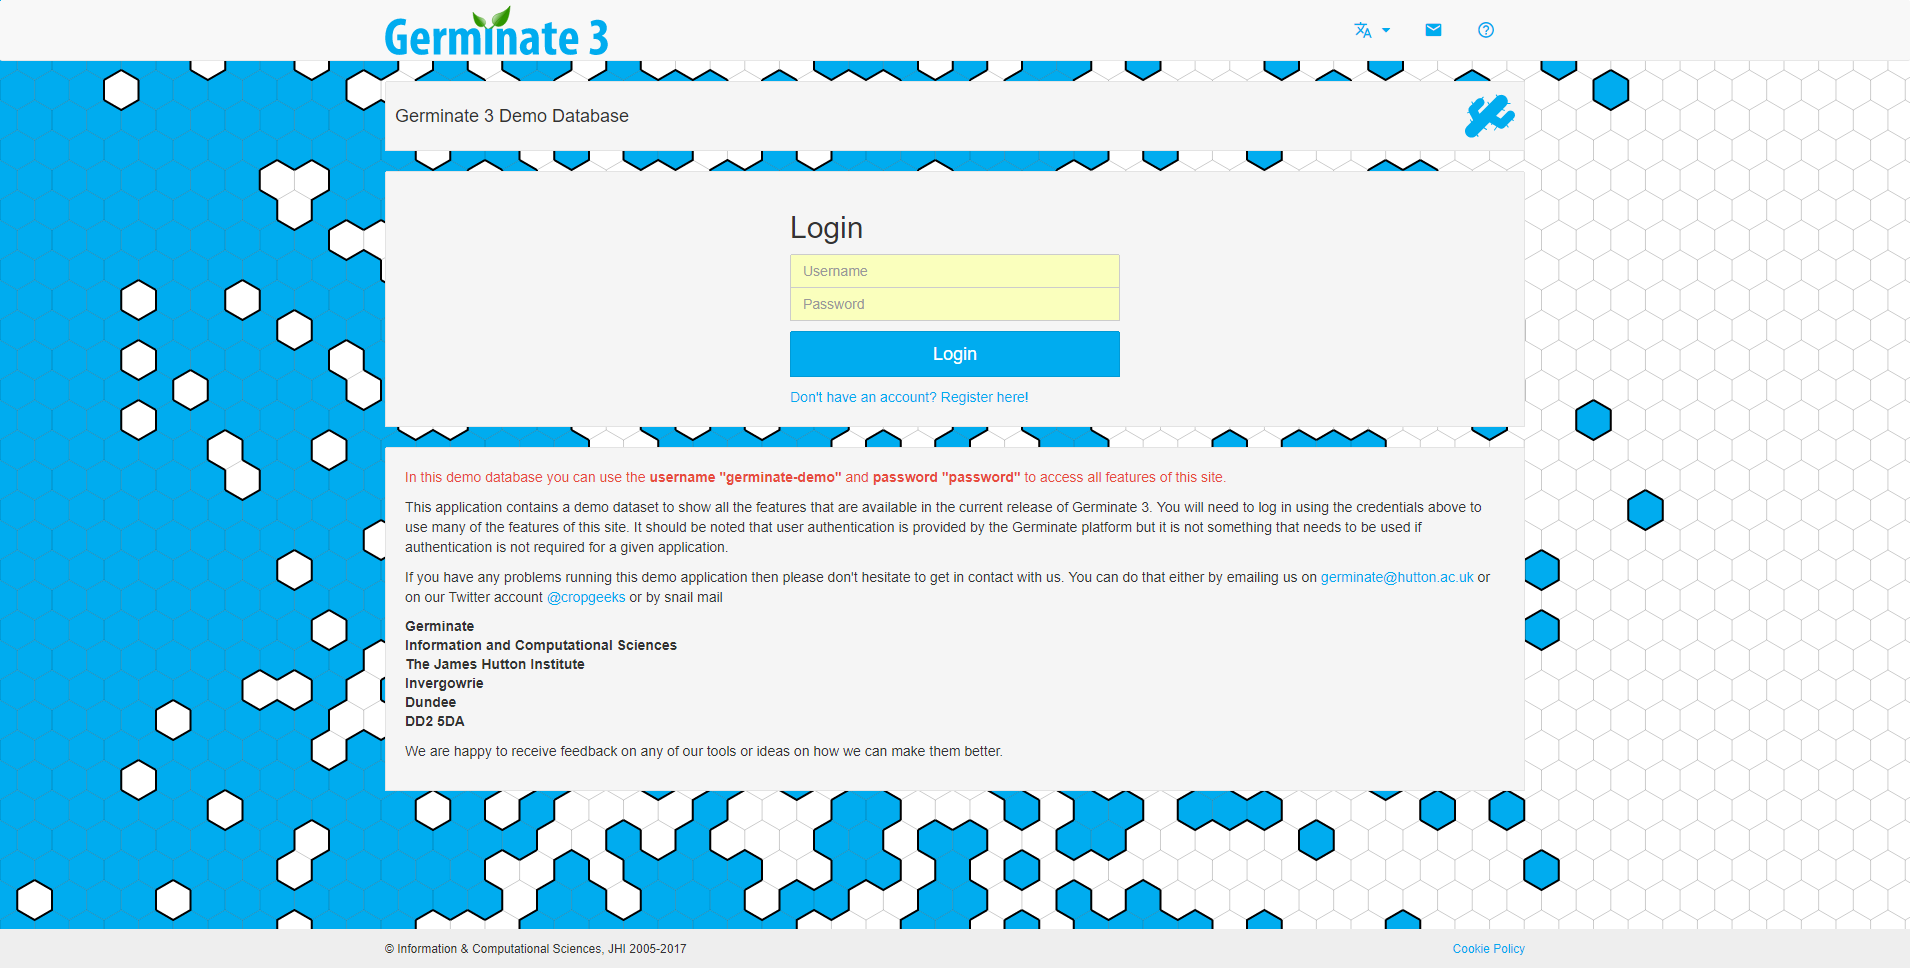
\includegraphics[width=0.85\linewidth]{img/overview/login.png}
	\caption{Depending on the configuration of {\germinate}, you may be asked to log in.}
	\label{fig:overview:login}
\end{figure}

\subsection{Page layout}
Figure \ref{fig:overview:home} shows the main layout of the {\germinate} web interface. The main menu of {\germinate} is positioned to the left (Figure \ref{fig:overview:home}A). It is used to navigate between pages. Submenus can be expanded by simply clicking on the items showing the caret symbol. The menu is explained in more detail in Section \ref{sec:features:menu}. The overall search feature, shown in Figure \ref{fig:overview:home}B, allows you to run a full-text search across the whole database. The results will be grouped into topical categories. See Section \ref{sec:features:search} for more details. The interface has a banner along the top containing the {\germinate} logo and a few dropdown menu items in the top right corner (\cf Figure \ref{fig:overview:home}C). These items include the language selector which will be covered in Section \ref{sec:features:language-selector}, social media buttons, the marked item lists covered in Section \ref{sec:features:marked-items}, a user menu with specific functions based on your type of account, a "contact us" button and, finally, a help button that can be clicked to get more information about the current page (\cf Section \ref{sec:features:help}). An overview of the number of database items for certain types is shown in Figure \ref{fig:overview:home}D. Recent news about both the {\germinate} interface and the contained data are available in the news section shown in Figure \ref{fig:overview:home}E. Finally, a section about other projects that are related to the project you are currently looking at are available in Figure \ref{fig:overview:home}F.

\begin{figure}
	\centering
	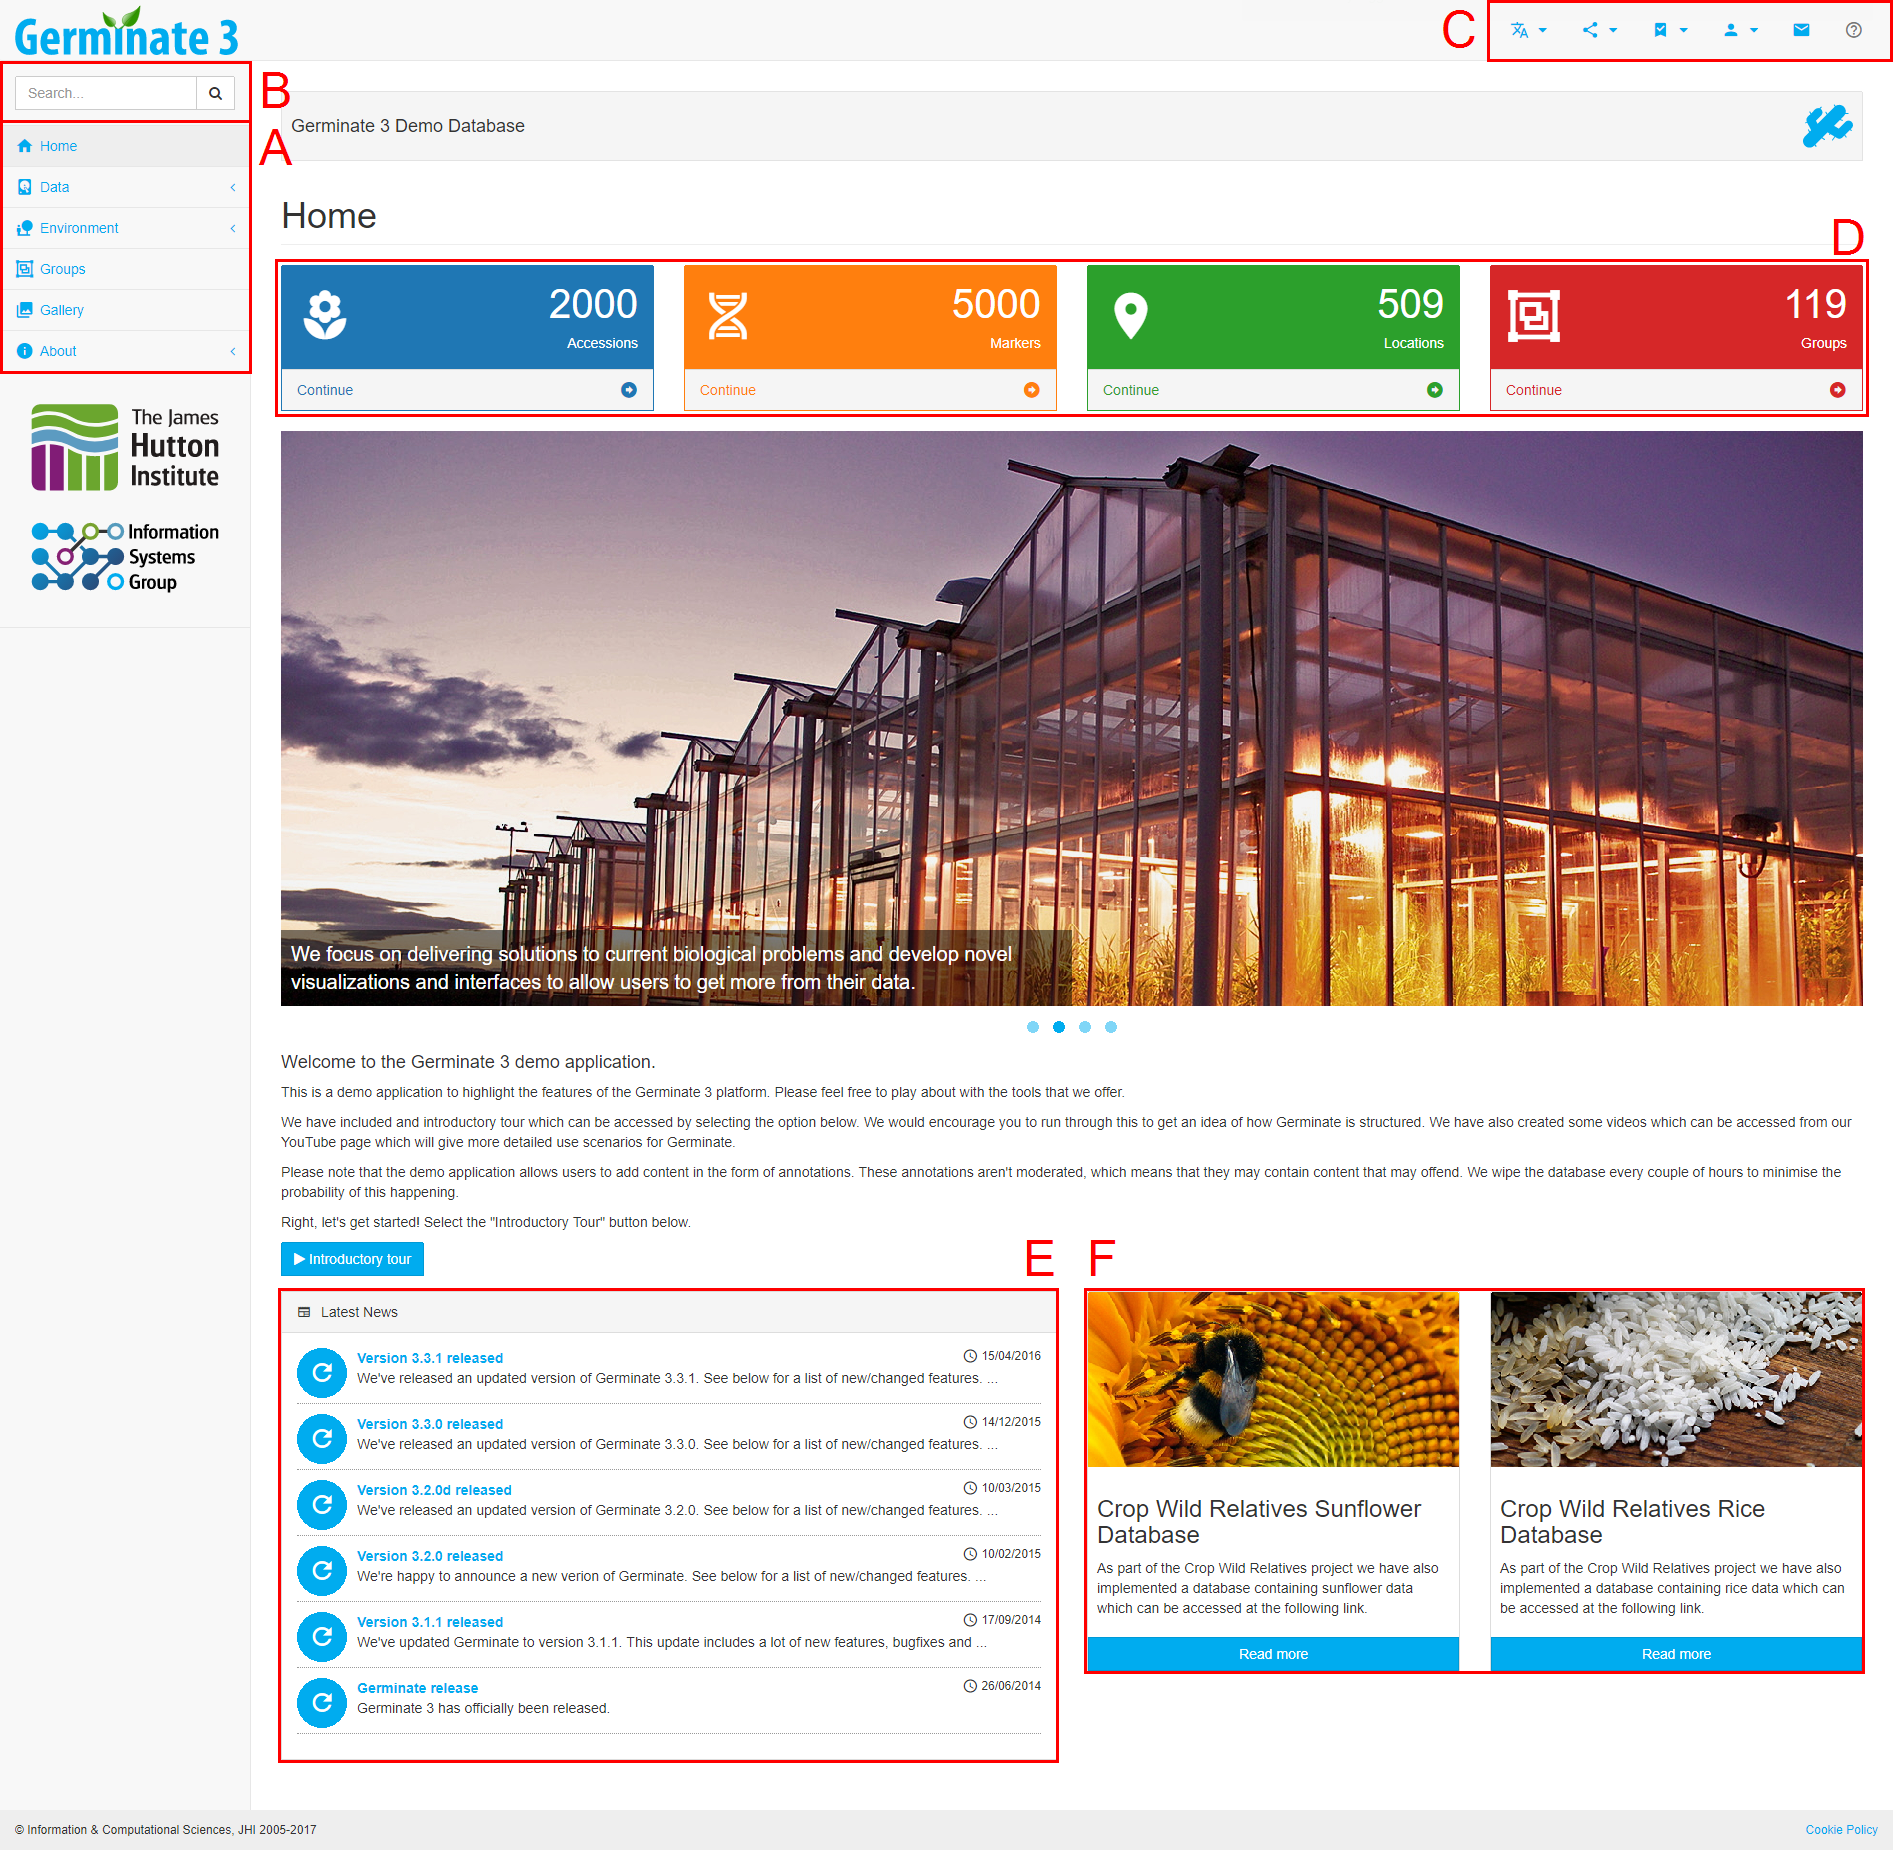
\includegraphics[width=0.85\linewidth]{img/overview/home.png}
	\caption{The home page of {\germinate} is the first page you will see. (A) The main menu of {\germinate} used to navigate the page. (B) The search box used for free-text searches of the database. (C) Language selector, social media buttons, marked item lists, user menu and the help button. (D) An overview of number of data objects that are stored in {\germinate}. (E) Latest news about this instance of {\germinate} and the contained data. (F) Other projects that have a relation to the current project.}
	\label{fig:overview:home}
\end{figure}
\section{Features}
In this section, we will highlight the main features of Germinate. This section will expand as we add new features.

\subsection{Internationalization and Localization}
\label{sec:features_i18n}
Germinate fully supports internationalization for an unlimited number of languages. Every text that you can see on the web interface can be localized. The language used on start-up is chosen based on the browser settings, but the user can easily switch to a different language by selecting it from the combo box at the bottom of the page. Have a look at Section \ref{sec:example_i18n} for usage details.

\subsection{Help}
Every page can include a help text. This text will be shown when the user clicks on the help icon. The main purpose of this help is to explain features of the current page to the user. As a result, the page itself does not look cluttered, but the user is still able to find help if the workflow of the page is not obvious.

\subsubsection{Tours}
In addition to a simple help text, we also offer the ability to add interactive tours to the pages. An interactive tour can be described as a sequence of help texts with visual feedback on the page itself. These steps can guide the user through the page and explain every step in detail. An example of a tour step can be seen in Figure \ref{fig:tour}.

\begin{figure}
    \centering
    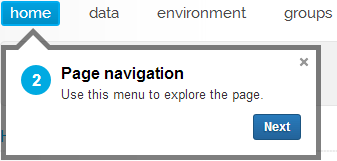
\includegraphics[scale=0.7]{img/features/tour-example2.png}
    \caption{Example step of a tour}
    \label{fig:tour}
\end{figure}

\subsection{News}
The Germinate web interface contains a place holder to show the latest news of the project. On the database side, these news are stored in two tables and can be updated at any time. The web interface will check the availability of news and show the three latest entries at the bottom of the page. Changes on the database side will immediately be visible on the website.

\subsection{Notifications}
Germinate offers a set of essential notification types. The notification system is based on Toastr \cite{Toastr}. All notifications fully support internationalization as well as custom styling. The currently available notification types can be seen in Figure \ref{fig:notification-types}. Section \ref{sec:example_notification} contains an example showing how to use the notification system.

\begin{figure}
    \centering
    \begin{subfigure}[t]{0.3\textwidth}
        
\includegraphics[width=\textwidth]{img/features/notification_success.png}
        \caption{Success}
    \end{subfigure}
    \hspace*{0.1\textwidth}
    \begin{subfigure}[t]{0.3\textwidth}
        
\includegraphics[width=\textwidth]{img/features/notification_error.png}
        \caption{Error}
    \end{subfigure}\\
    \begin{subfigure}[t]{0.3\textwidth}
        
\includegraphics[width=\textwidth]{img/features/notification_warning.png}
        \caption{Warning}
    \end{subfigure}
    \hspace*{0.1\textwidth}
    \begin{subfigure}[t]{0.3\textwidth}
        
\includegraphics[width=\textwidth]{img/features/notification_info.png}
        \caption{Info}
    \end{subfigure}
    \caption{Available notifications}
    \label{fig:notification-types}
\end{figure}

\subsection{Available pages}
\label{sec:pages}
This section gives an overview of all the pages that are available for Germinate. Based on your requirements and the data that is available, you can decide which pages should actually be available on the web interface and hide all others. The set of available pages can be changed dynamically without having to re-deploy the application. This gives you the freedom to customize your Germinate experience just as you please.

A table with the available pages can be found in Table \ref{tab:pages}.

\begin{longtable}{p{\dimexpr 0.27\linewidth-2\tabcolsep}p{\dimexpr 0.45\linewidth-2\tabcolsep}p{\dimexpr 0.28\linewidth-2\tabcolsep}}
	%\caption{List of all available pages in Germinate 3}\\
	\toprule
	\textbf{Page name}     & \textbf{Description} & \textbf{Required data} \\
	\midrule\midrule
	\endhead
	about-germinate        & Shows information about Germinate & - \\ \midrule
	about-project          & Shows information about the project & - \\ \midrule
	accessions-for-collsite & Shows available accessions for the selected collecting site & \cellwrap{germinatebase,\\locations,\\locationtypes,\\countries}\\ \midrule
	acknowledgements       & Shows acknowledgements & - \\ \midrule
	allele-freq-dataset & Shows the datasets containing allele frequency data & \cellwrap{datasets,\\datasetstates,\\datasetpermissions,\\experiments} \\ \midrule
	allele-freq-export  & Page showing the settings used for the export of allele frequency data & \cellwrap{allelefrequencydata,\\datasets,\\datasetstates,\\datasetpermissions,\\germinatebase,\\groups,\\groupdatasets\\grouptypes,\\maps} \\ \midrule
	allele-freq-result  & Page showing the result of the allele frequency data export & \cellwrap{allelefrequencydata,\\datasets,\\datasetstates,\\datasetpermissions,\\groups,\\maps} \\ \midrule
	browse-accessions       & A paginated table containing all the accessions in the database. & \cellwrap{countries,\\germinatebase,\\locations,\\taxonomies,\\subtaxa} \\ \midrule
	cart                   & The cart contains marked accessions. & \cellwrap{germinatebase} \\ \midrule
	categorical-datasets    & Shows the datasets containing categorical data & \cellwrap{datasets,\\datasetstates,\\datasetpermissions,\\experiments} \\ \midrule
	categorical-export      & Page showing the settings used for the export of categorical data & \cellwrap{datasets,\\datasetstates,\\datasetpermissions,\\germinatebase,\\groups,\\groupdatasets,\\grouptypes\\phenotypes} \\ \midrule
	climate                & Page showing the settings used for the export of categorical data & \cellwrap{climatedata,\\climates,\\groups,\\units,\\groups,\\grouptypes,\\phenotypes} \\ \midrule
	collsite-treemap        & Page showing a treemap of the collectingsites & \cellwrap{countries,\\germinatebase,\\locations} \\ \midrule
	cookie                 & Page showing the cookie policy & - \\ \midrule
	dataset-overview       & Page showing all the available datasets & \cellwrap{datasets,\\datasetstates,\\datasetpermissions,\\experiments,\\experimenttypes} \\ \midrule
	experiment-details     & Page showing all datasets that are part of an experiment & \cellwrap{datasets,\\datasetstates,\\datasetpermissions,\\experiments,\\experimenttypes} \\ \midrule
	gallery                & A gallery of images & \cellwrap{images,\\imagetypes} \\ \midrule
	genotype-datasets       & Shows the datasets containing genotypic data & \cellwrap{datasets,\\datasetstates,\\datasetpermissions,\\experiments} \\ \midrule
	genotype-export         & Page showing the settings used for the export of genotypic data & \cellwrap{datasets,\\datasetstates,\\datasetpermissions,\\genotypes,\\germinatebase,\\groups,\\groupdatasets\\grouptypes,\\mapdefinitions,\\maps,\\markers} \\ \midrule
	geographic-search       & Page used to query for collecting sites by distance to a query location & \cellwrap{countries,\\locations} \\ \midrule
	geography              & Page that shows different visualizations of collecting sites on maps & \cellwrap{countries,\\locations} \\ \midrule
	groups				   & Page listing defined groups of accessions, markers, ... & \cellwrap{groupmembers,\\groups,\\grouptypes} \\ \midrule
	help				   & Page with general help information & - \\ \midrule
	home				   & Welcome page of the web interface & - \\ \midrule
	login                  & The login page of Germinate & - \\ \midrule
	logout				   & The logout page of Germinate & - \\ \midrule
	map-details			   & Page listing the details about a selected map & \cellwrap{mapdefinitions,\\mapfeaturetypes,\\maps,\\markers} \\ \midrule
	marker-details          & Page listing the details about a selected marker & \cellwrap{datasets,\\genotypes,\\markers} \\ \midrule
	mega-environments       & Page with the mega environments & \cellwrap{countries,\\germinatebase,\\locations,\\megaenvironmentsdata,\\megaenvironments,\\megaenvironmentsource,\\soils}\\ \midrule
	news				   & List of the latest news & \cellwrap{news,\\newstypes} \\ \midrule
	passport			   & Page listing the details about a selected accession & \cellwrap{countries,\\germinatebase,\\locations,\\subtaxa,\\taxonomies} \\ \midrule
	search				   & Shows search results & \cellwrap{countries,\\germinatebase,\\locations,\\markers,\\mapdefinitions,\\mapfeaturetypes} \\ \midrule
	trials                 & Page with different visualizations of trials data & \cellwrap{germinatebase,\\phenotypes,\\trialsdata} \\ \midrule
	trials-datasets         & Shows the datasets containing trials data & \cellwrap{datasets,\\datasetstates,\\datasetpermissions,\\experiments} \\ \midrule
	trials-individual       & Shows visualizations of trials data for an accession and a phenotype & \cellwrap{trialsdata,\\trialseries,\\trialsites} \\ \midrule
	\bottomrule
	\label{tab:pages}
\end{longtable}

\subsubsection{User registration}
\label{sec:registration}

Germinate can be used with and without authentication. This means that you can decide if you want to restrict access to your Germinate instance to registered users. If you decide to do so, you'll need people to be able to register. The registration form of Germinate (Figure \ref{fig:user_registration_registration}) provides a concise and easy way to register. If you choose to use a disclaimer that potential new users have to accept, this will appear before the form is visible. Once the user completes the form, they will either get access right away or you need to approve the new users manually. This is based on the setting of the property \texttt{Gatekeeper.Registration.Needs.Approval} (see Section \ref{sec:config-properties} for help). If you choose to use the approval approach, you'll see the screen shown in Figure \ref{fig:user_registration_approval} after selecting "Approve users" in Gatekeeper. The user will be notified with your decision.

\begin{figure}
    \centering
    \begin{subfigure}[b]{0.475\textwidth}
        \centering
        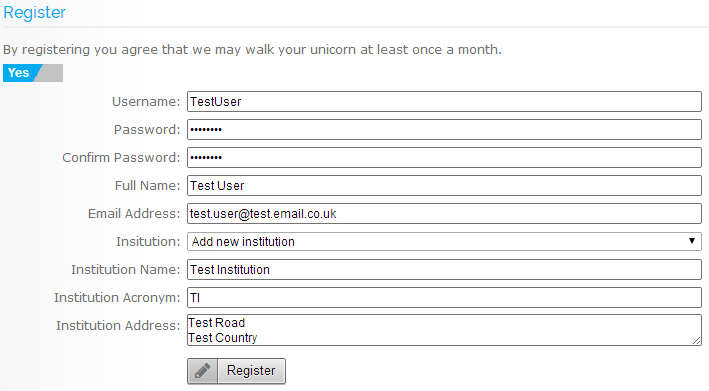
\includegraphics[width=1.0\textwidth]{img/features/registration.png}
        \caption{Registration form on the Germinate 3 site}
        \label{fig:user_registration_registration}
    \end{subfigure}
    \hspace*{0.5cm}
    \begin{subfigure}[b]{0.475\textwidth}
        \centering
        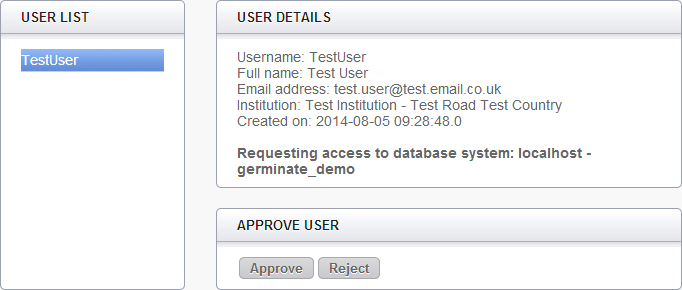
\includegraphics[width=1.0\textwidth]{img/features/registration-approve.png}
        \caption{Approval page on the Gatekeeper page}
        \label{fig:user_registration_approval}
    \end{subfigure}
    \caption{User registration}
    \label{fig:user_registration}
\end{figure}

\subsubsection{Groups}
Germinate allows you to define groupings of various items which makes exporting or visualizing data more comfortable. An intuitive example of groups are accession groups. A group of accessions can contain accessions that are similar to each other or a list of accessions that you want to export against a map for visualization in Flapjack.

A new group can be created with a couple of clicks: First, select the type of group that you want to create, \eg accession group, collecting site group, marker group etc. Afterwards, create a new group by just entering the name of the new group.

To delete group members, just select the group that you want to modify and check the items to remove in the table. Afterwards click on the delete button below the table. To delete a complete group, click on the delete icon next to the group selection box.

\paragraph{Searching by item criteria}
Searching for the items you want to add to the group is very straight forward. Germinate supports searching on almost all columns of the table containing the data. Examples are: "country of origin", "region", "state, "latitude", "longitude" and "elevation" for collecting sites. You can restrict your search by specifying multiple criteria. The criteria currently have the following structure:
\begin{center}
    <column> \{less than, greater than, equal\} <value>
\end{center}
\noindent
Multiple criteria can be combined using logical conjunction ($\land$, AND) and disjunction ($\lor$, OR). Note that conjunction binds stronger than disjunction making the order of criteria important. An example can be seen in Figure \ref{fig:group_search} (\subref{fig:group_search_item}). The example requests all accessions with "mexico" as their country of origin \textbf{or} those accessions with a name starting with "A".

\paragraph{Searching by climate criteria}
If climate data is available, Germinate allows to select subsets of items based on a combination of climate criteria. The process is identical to the one seen above. Figure \ref{fig:group_search} (\subref{fig:group_search_climate}) shows an example. The example requests collecting sites having a maximal average temperature of less than 30 \textbf{and} having a minimal average temperature of more than 20.

\begin{figure}
    \centering
    \begin{subfigure}[t]{1.0\textwidth}
        \centering
        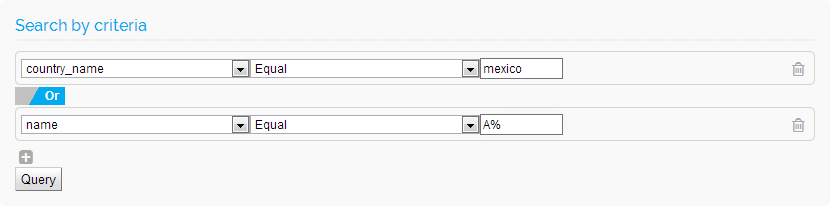
\includegraphics[scale=0.5]{img/features/groups_item.png}
        \caption{Accession search by item criteria}
        \label{fig:group_search_item}
    \end{subfigure}
    \\
    \begin{subfigure}[t]{1.0\textwidth}
        \centering
        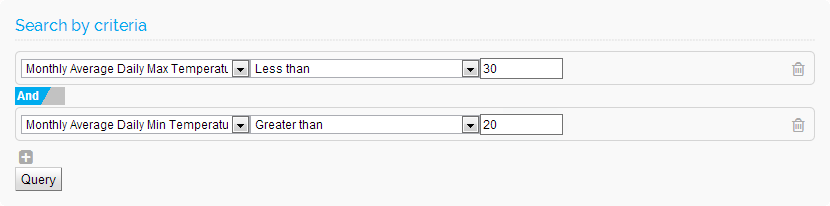
\includegraphics[scale=0.5]{img/features/groups_climate.png}
        \caption{Collecting site search by climate criteria}
        \label{fig:group_search_climate}
    \end{subfigure}
    \caption{Examples of group searches}
    \label{fig:group_search}
\end{figure}

\subsubsection{Data}
The main purpose of Germinate is to store multiple data types, let the user query them and create visualizations of the data. In this section, we will give an overview of the different data types and visualizations Germinate supports.

\paragraph{Browse accessions and Passport}
This page lists all accessions stored in Germinate in a tabular format. The table is sortable and supports pagination, \ie it will split into multiple pages if necessary to ensure readability. Clicking on an accession will take you to the passport page. The passport page contains all the meta information that is available for the selected accession such as name, genus, breeder information, images and annotations.

Passport data tends to be quite fragmented so its perfectly possible that we have limited data for some lines while others have a full complement.

\paragraph{Maps and Markers}
The map page shows a list of available maps defined in Germinate. Clicking on a map will show its member markers with detailed information about chromosome and position on the chromosome. In turn clicking on a marker shows information about the molecular and genotype information about this marker as well as a list of the datasets the marker is contained in. Click on the dataset to reveal the genotypes for the selected combination of marker and dataset.

\paragraph{Genotype data export}
The genotype information held in Germinate can be exported as tab separated values as well as in a format that is compatible with the genotype data viewer \textit{Flapjack}. The process of exporting the data is structured like a wizard dialog.

First you need to select the dataset containing the data that you want to export. The second wizard page shows the accession and marker groups as well as the maps that are visible to you. Just select the items that you want to export. The \textit{Crap Data Filter} (CDF) can be enabled to prune markers from the export that exceed a certain threshold for missing or heterozygous values.
Finally, you need to select the file containing the raw data. The third page finally contains your exported data in both already mentioned formats. If the CDF was enabled, this page will show the list of deleted markers for your convenience.\\
\\
\textbf{Note}: Make sure that all the files that contain your genotype data are encoded with UTF-8.

\paragraph{Allele frequency data export}
Exporting allele frequency data is almost identical to the genotype data export. The first two wizard pages are again used to select datasets and accession and marker groups. The third page differs from the genotype export, because this is the page where you actually can decide how you want your data to be binned. The binning step is necessary for visualization in Flapjack. Currently, there are three types of binning mechanisms: \textit{Equal-width binning}, \textit{Split point binning} and \textit{automatic binning}.

Equal-width binning will result in a specified number of bins all having the same width. Split point binning is an extension of this principle. It lets you specify a split point and a number of bins to either side of the split point. The parts to the left and the right of the split point are binned according to the equal-width binning principle. Automatic binning is more sophisticated. It will automatically determine the best splitting points given a number of bins. The resulting binning will contain approximately the same number of items in each bin. Another name for this principle is consequently equal-size binning.

\paragraph{Phenotype data export}
The phenotype export process is structured similarly to the genotype export. In the first step you can select the dataset containing your data. The next page will show the available phenotypes and accession groups that can be selected for export.

Now you can select if you just want to have a look at the data or if you want to be able to download it as well. Check the checkbox at the bottom of the page to create a downloadable file containing the data. Pressing continue will start the export process. Once the date is returned from the server, it will be displayed at the bottom of the page. A download link will be attached below the table if you decided to select data download in the previous step.

\subsubsection{Environment}
Environmental data can include climate data, GIS (Geographic information system) data, soil data and many more. Germinate can store all that information and use it to create meaningful visualizations and overviews.

\paragraph{Geography}
The geography page visualizes the geographic data contained in Germinate on Google Maps. So far the only instance that holds geographic information are the collecting sites, for which we store latitude, longitude and altitude information.

There are three types of maps that are currently supported. The first type is a simple map with a marker for each data point in the database. This can get quite cluttered when the number of items increases. The two other types of maps pose solutions to this issue.

The first of them is a \textit{Heatmap Layer} \cite{HeatmapLayer} for the map. A heatmap is a data visualization technique where the data points are not represented individually, but instead they are used to calculate a density function which is then plotted on top of the Google Map. The density function assigns a high value to areas where the probability of observing data points is high and a low value to areas where this probability is low. To visualize this principle, the heatmap is color-coded.

The other alternative to individual markers is the \textit{MarkerClusterer} \cite{MarkerClusterer}. The MarkerClusterer uses a very basic grid-based clustering algorithm to group clusters located in the same area into clusters. This solution massively reduces the number of visible markers on the screens since each cluster is now represented by a marker instead of the hundreds of actual markers it contains. The clusters will be re-generated on every zoom level resulting in approximately the same number of visible clusters independent of the zoom level.

Figure \ref{fig:geography-maps} shows an example dataset containing about 1000 markers. Figure \ref{fig:geography-maps}(a) shows the individual markers and we can see that this is very cluttered. Figure \ref{fig:geography-maps}(b) and \ref{fig:geography-maps}(c) show the HeatmapLayer and MarkerClusterer respectively. 

\begin{figure}
    \begin{subfigure}[t]{0.32\textwidth}
        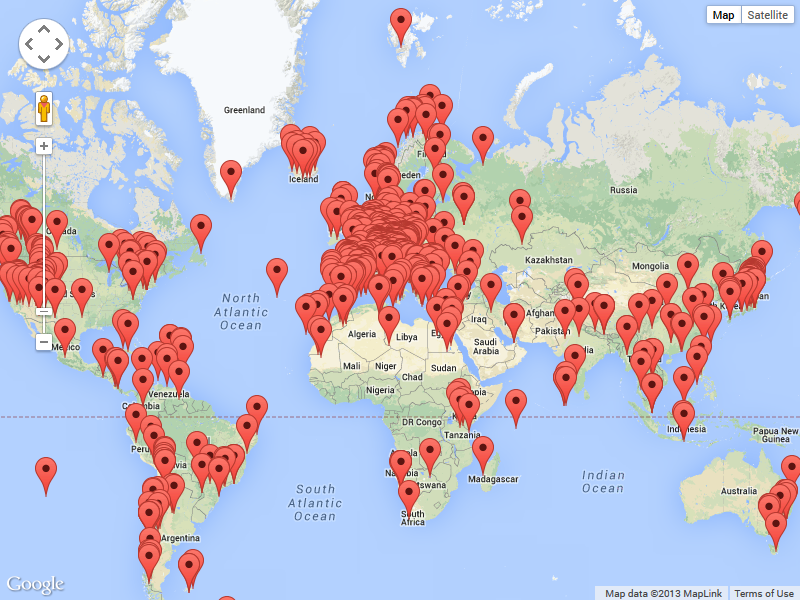
\includegraphics[width=\textwidth]{img/features/markers.png}
        \caption{Markers}
    \end{subfigure}
    ~
    \begin{subfigure}[t]{0.32\textwidth}
        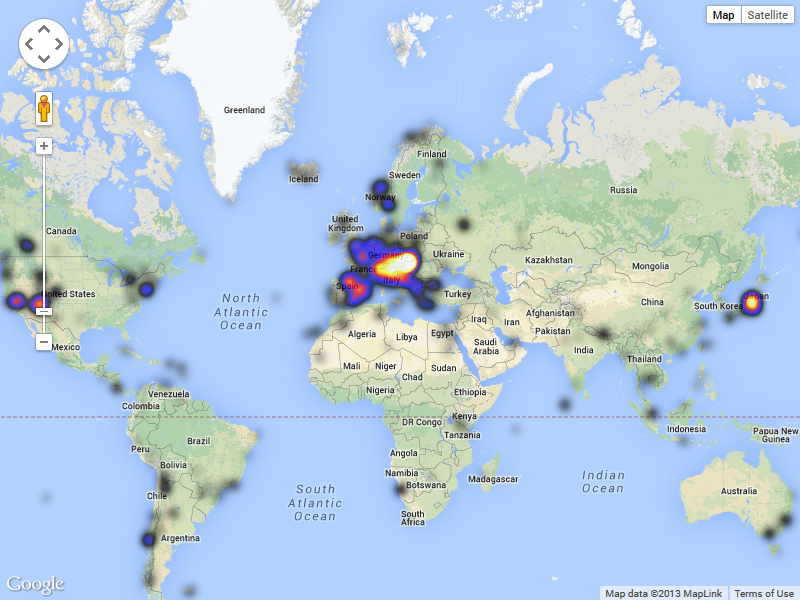
\includegraphics[width=\textwidth]{img/features/heatmap.png}
        \caption{HeatmapLayer}
    \end{subfigure}
    ~
    \begin{subfigure}[t]{0.32\textwidth}
        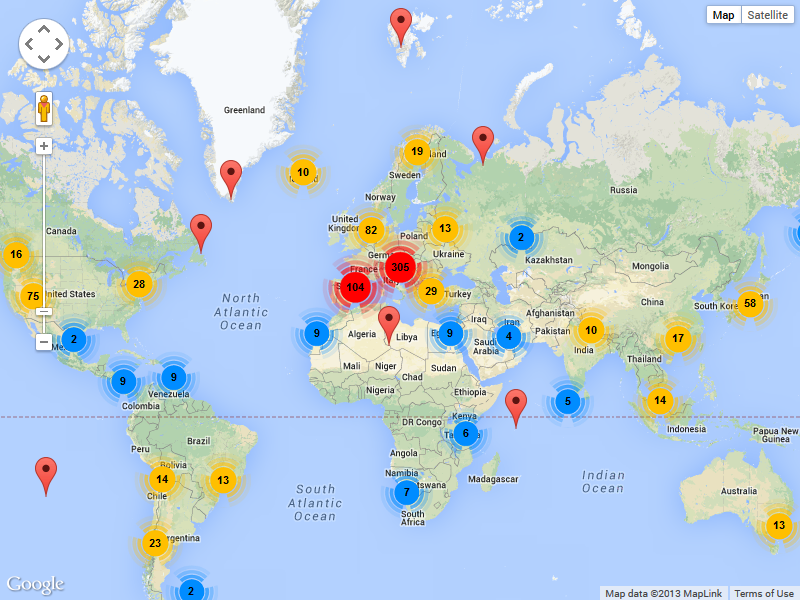
\includegraphics[width=\textwidth]{img/features/markerclusterer.png}
        \caption{MarkerClusterer}
    \end{subfigure}
    \caption{Different representations of the same geographic information}
    \label{fig:geography-maps}
\end{figure}

\paragraph{Geographic Search}
The geographic search can be used to find collecting sites with the help of a Google Map. You can either enter coordinates (latitude and longitude) directly, or scroll to the position of interest on the map. A click on the "Continue" button will list all collecting sites ordered by their distance (in km) to your query location.

\paragraph{Geographic Treemap}
Treemapping (\url{http://en.wikipedia.org/wiki/Treemapping}) is a method for displaying hierarchical data by using nested rectangles. In our case, we visualize the hierarchy of locations in a treemap. The highest level of abstraction can be defined using the \texttt{Germinate\allowbreak .CollectingsiteTreemapColumn} property described in Section \ref{sec:config-properties}. Clicking on one of the top level rectangles will zoom in and show the actual collecting sites. Clicking on those will take you to a page listing all the accessions collected at this site.

\paragraph{Mega Environments}
A mega environment can be defined as a set of areas sharing the same or very similar attributes ranging from biotic and abiotic stresses to customer preferences.

The mega environments page lists all recorded mega environments with the collecting sites located within them. Selecting a collecting site takes you to a page showing the accessions found at this site.

The data contained in both the mega environment page as well as the collecting sites page can be downloaded in KML (\textbf{K}eyhole \textbf{M}arkup \textbf{L}anguage) format allowing viewing in Google Earth \cite{GoogleEarth}.

\paragraph{Climate}
Climate data is very diverse. Everything that can be measured by sensors can be considered as climate information. Examples are precipitation, hours of daylight, temperature, frost frequency and atmospheric pressure. Germinate can store all kinds of climate data. The climate page of the Germinate web interface visualizes the contained data in a compact and understandable way. Figure \ref{fig:climate_table} shows an example visualization using color-coding of the average measured temperature for the given collecting sites.

If you have climate layer images that go along with your climate data, Germinate is able to display them on top of a Google Map below the climate chart.

\begin{figure}
    \centering
    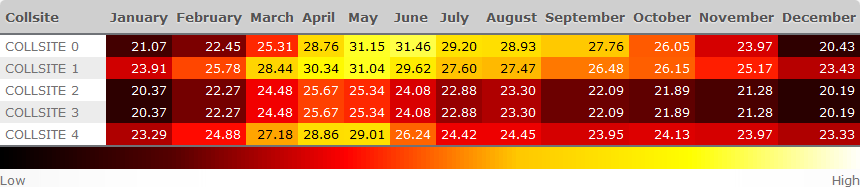
\includegraphics[scale=0.5]{img/features/climate_table.png}
    \caption{Color-coded climate table (average temperature in \textcelsius)}
    \label{fig:climate_table}
\end{figure}

\subsubsection{Image gallery}
The image gallery is an elegant way to display images that do not fit on any of the other pages. The images will be held in a table structure and can be browsed in a pagewise fashion. New images can easily be added by copying them into the following directory:
\begin{center}
    \texttt{<Apache Directory>/webapps/<project.name>/WEB-INF/classes/download}
\end{center}
There are two sub-folders called \texttt{images} and \texttt{thumbnails}. Copy the full size images into the \texttt{images} directory and small thumbnails into the \texttt{thumbnails} folder. For optimal visual appearance make sure that all the thumbnails have the same height. A height of 150px is a good reference value.

The images will be sorted by the "Last Modified Date" making sure that the newest images appear first.

\subsubsection{Search}
Every website should have a basic search feature. The search feature of Germinate allows to search for accessions, collecting sites, markers etc. by their features. You know the name of an accession? Excellent, just search for it and tell Germinate that it's the name you're searching for. Only know the ID? No problem, just use the ID instead and mark it as the ID. We use \texttt{\%} as the wildcard character. A wildcard character can be used to substitute for arbitrary other characters. As an example, \texttt{\%king\%} will match \texttt{United Kingdom}, whereas \texttt{king\%} will only match \texttt{Kingdom}. Note that we currently don't match cases during the search.

\subsection{Color Themes}
Germinate is highly customizable. We have already seen a lot of configuration options in Section \ref{sec:config-properties}. In this section we want to highlight one of the customization features in particular: color themes. The configuration properties responsible for the color theme of Germinate are:

\begin{lstlisting}[style=Properties]
Germinate.Template.HighlightColor=<main color of all highlights on the interface>
Germinate.Template.CategoricalColors=<colors used for some of the charts>
\end{lstlisting}

\noindent
We will now show how the look of Germinate can be completely changed by just setting these two properties. The default color theme of Germinate is a composition of different shades of blue (see Figure \ref{subfigure:blue-theme}). With the following property changes, we get the completely changed theme seen in Figure \ref{subfigure:red-theme}.

\begin{figure}[h]
	\centering
	\begin{subfigure}[t]{0.48\textwidth}
		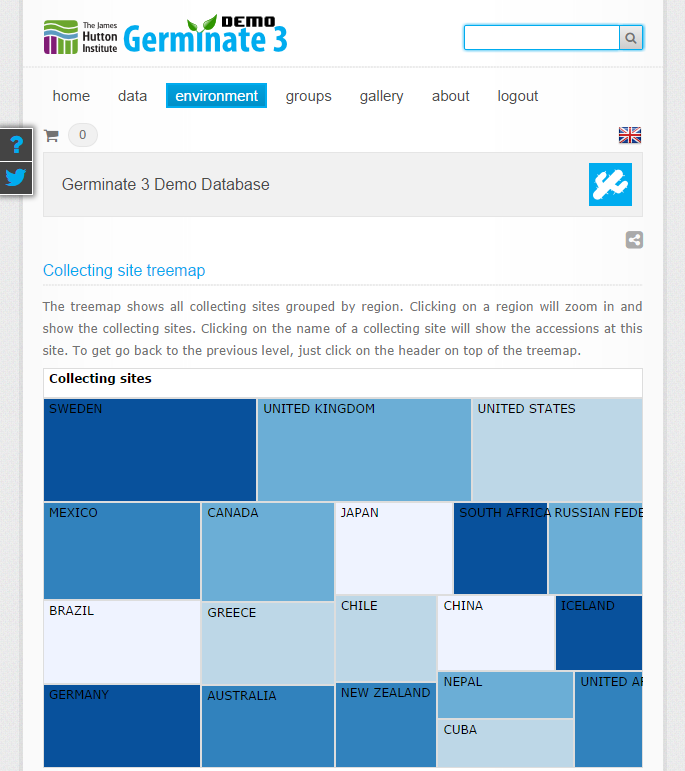
\includegraphics[width=\textwidth]{img/features/themes-blue.png}
		\caption{Default blue color theme}
		\label{subfigure:blue-theme}
	\end{subfigure}
	~
	\begin{subfigure}[t]{0.48\textwidth}
		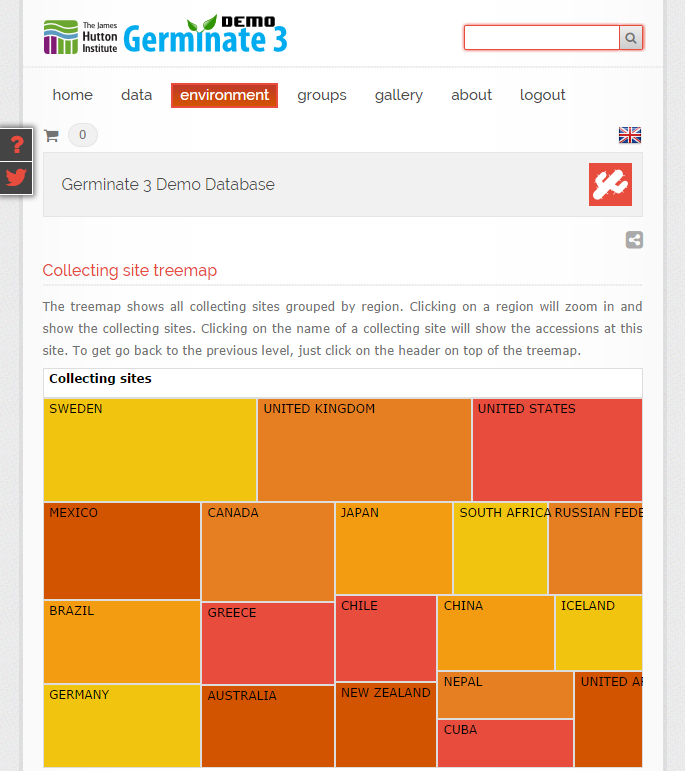
\includegraphics[width=\textwidth]{img/features/themes-red.png}
		\caption{Red color theme}
		\label{subfigure:red-theme}
	\end{subfigure}
	\caption{Different color themes}
	\label{fig:color-themes}
\end{figure}

\begin{lstlisting}[style=Properties]
Germinate.Template.HighlightColor=#e74c3c
Germinate.Template.CategoricalColors=#e74c3c,#d35400,#e67e22,#f39c12,#f1c40f
\end{lstlisting}

\noindent As you can see, the color theme affects almost all elements of the website: links, headings, backgrounds, icons, highlight effects, chart colors, etc.

Although we do our best to take care of all elements, we can't simply change the images you include, \ie the included images do not change colors based on these settings. An example is the Germinate 3 logo in both screenshots. As can be seen, it stays blue. However, all other elements that are included in the default installation of Germinate will change color according to the defined properties.

\subsection{Security}
\label{sec:example_security}
As already mentioned earlier, Germinate is equipped with a secure login system\footnote{Germinate is only as secure as the connection between client and server. Use a secure connection (TLS/SSL) to prevent password snooping.}. This feature is completely optional, but it allows you to protect your data from any unauthorized access. In this section, we will explain how the security system works and we will show what is necessary to use it properly.

\begin{figure}[h]
    \centering
    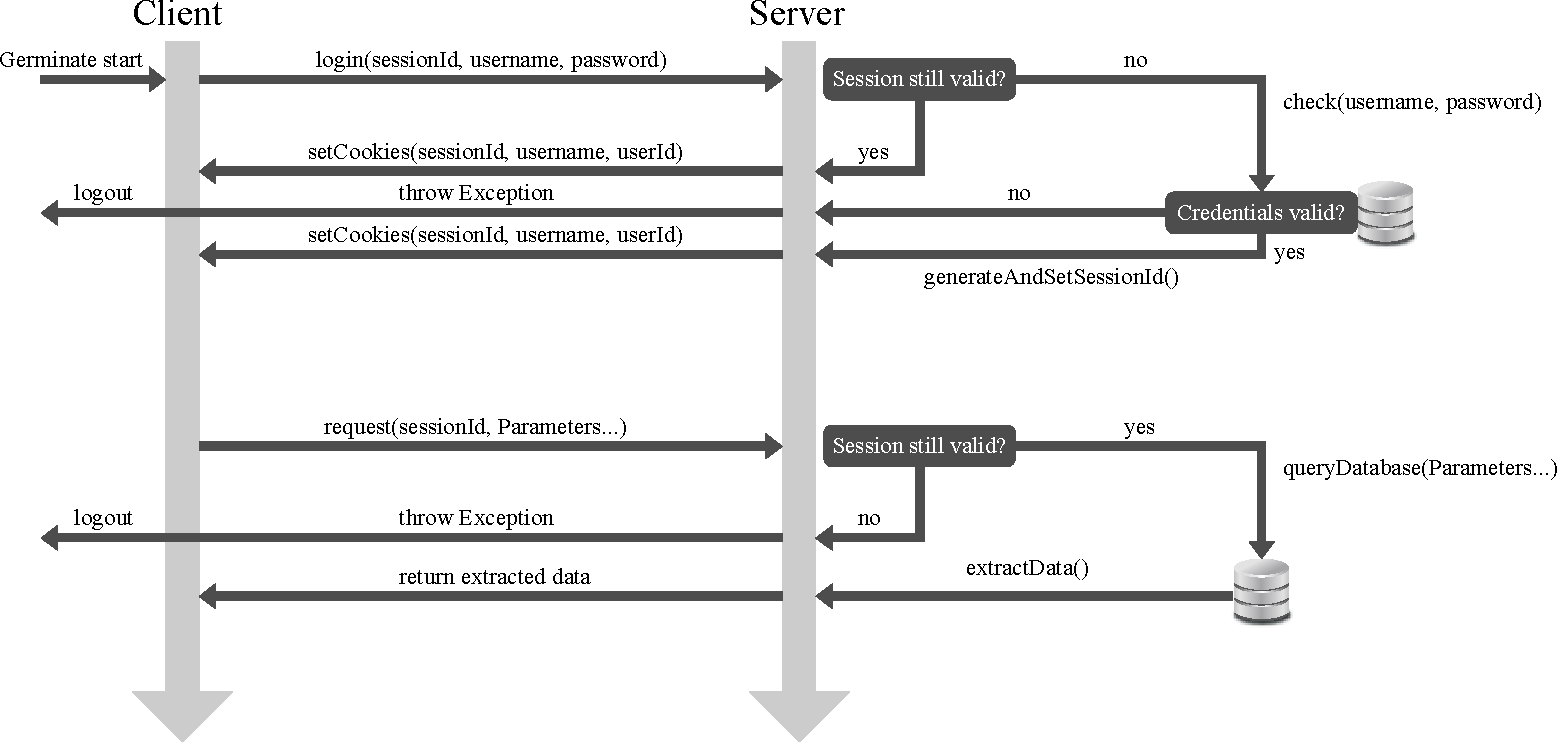
\includegraphics[scale=0.5]{img/examples/authentication.pdf}
    \caption{Authentication procedure of Germinate}
    \label{fig:authentication}
\end{figure}

Figure \ref{fig:authentication} shows the authentication process of Germinate. The figure contains two major parts. The upper part visualizes the login process, which is initialized by the user entering his/her credentials. These are sent to the server alongside any session id that is still stored in the client from previous sessions. The server will then check the session id that is received. If the id is still valid, the server will store the session id and return it to the client, which, in turn, will create a cookie containing this id.

If the session id is invalid, the server will check if the username password combination is genuine. This is done by encrypting the password and checking it against the entry in the database. If this check fails, the user will be logged out. Otherwise, the server will create a new session id, store it in the HTTP session and return it to the client, which will create a new cookie using this id. The login process is now complete and both the server (via HTTP session) and the client (via cookie) know the current session id.

For each new request that is made from the client, it will need to send the session id as the payload, \ie each remote procedure call (RPC) has to request the session id as a parameter to ensure the security of the communication. As a consequence if this, the server will receive the session id three times per request, namely via the HTTP session, via the cookie and via the payload. If all of these ids match up, the server can fulfil the client's request and return the data. However, if it fails, the user will be logged out.

As a final remark: Even if you currently do not want to enable the security feature, you should still write your code in a way that ensures it will work properly even when the security feature is enabled. Otherwise you might end up with a security leak.
\section{Data Types}
The following section will describe each data type that Germinate can handle in more detail. We will describe both the web interface that is used to display this data as well as what the export formats for each of the types are.

\subsection{Passport Data}

\subsubsection{Multi-Crop Passport Descriptors}
The Multi-Crop Passport Descriptors (MCPD) \cite{mcpd} is a widely used international standard to facilitate germplasm passport information exchange defined by the FAO. Germinate is fully MCPD V.2.1 compatible. The MCPD standard is used by many genebanks and genetic resources tools and utilities.

\subsection{Genotypic Data}
When we talk about genotypic data in the context of Germinate, we are referring to Single Nucleotide Polymorphic (SNP) or Simple sequence repeat (SSR) data. The data export process is shown in Figure \ref{fig:features:group-subselection}. After selecting the dataset you want to export, you can decide which accessions and markers should be included in the output. Data can be exported against different maps (cf. Section \ref{sec:features:genotypic-maps}), e.g. physical vs. genetic marker positions.

The data is exported into a tab-delimited text format as well as Flapjack \cite{flapjack} format. Figure \ref{fig:features:genotypic-data-flapjack} shows an example of data exported from Germinate visualized in Flapjack.

\begin{figure}
	\centering
	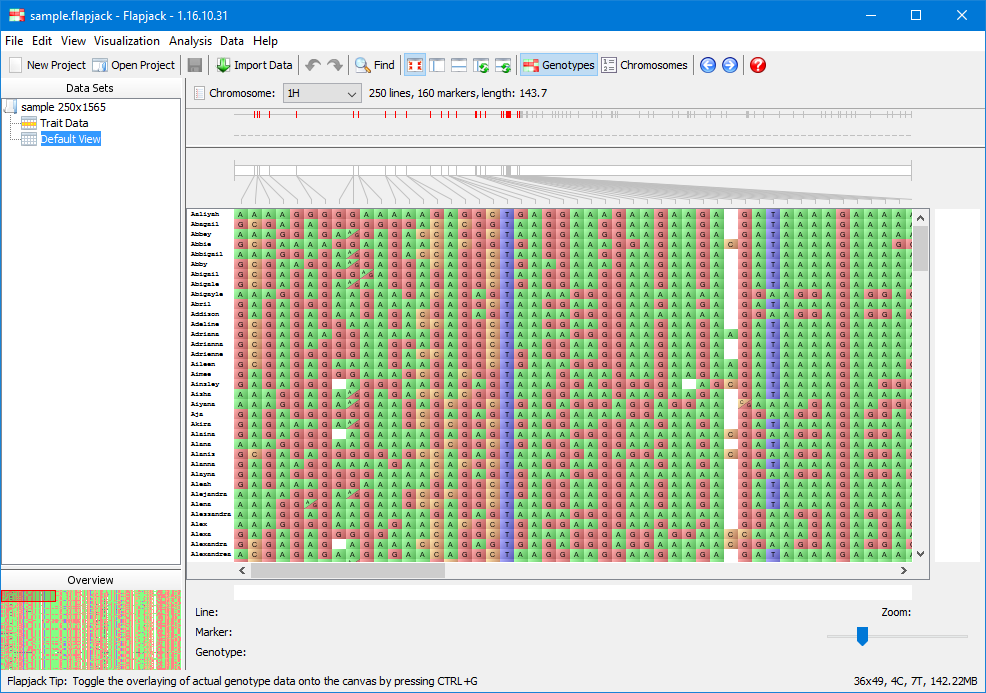
\includegraphics[width=0.85\linewidth]{img/features/genotypic-data-flapjack.png}
	\caption{Genotypic data exported from Germinate and visualized in Flapjack.}
	\label{fig:features:genotypic-data-flapjack}
\end{figure}

\subsubsection{Allele Frequency Data}
\todo{Paul}

\subsubsection{Genotypic Maps}
\label{sec:features:genotypic-maps}

\subsubsection{Genetic Markers}

\subsection{Phenotypic Trials Data}
Phenotypic data is a big part of Germinate. We put a lot of effort into developing meaningful visualizations as well as functionality and interoperability with our other software tools. 

After selecting a dataset (or multiple datasets), you will have the choice between different visualizations and the data download. The first tab shows an overview over the data within the selected datasets, whereas the second tab lets you plot two phenotypes against each other in a scatter plot. This is particularly useful to see if there is any correlation between them. Hovering over data points shows the values per dimension as well as the accession that is responsible for this data point. Clicking on this data point will take you to the passport page for this accession. You can draw a shape around data points of interest by clicking and dragging the mouse across the chart. This will highlight the data points within the shape. You can then either right-click or use the icon in the top right of the chart to add/remove these items to/from the marked item list.

\subsection{Climate Data}

\subsection{Chemical Compound Data}

% add the bubliography (without file extension) and style it
\bibliography{cite}
\bibliographystyle{unsrt}

\end{document}